\chapter{Choosing a filter}
\label{ch:choosing}

All the filters of this book have now run on the same robot and the same
data. This chapter collects the results of the showdown notebook, draws
the practical conclusions, and closes with the bridge from filtering to
the smoothing view used by modern localisation and mapping systems.

\section{The showdown}

Each scenario is repeated over several random seeds. A filter is
\emph{lost} when its median position error over the last 50 steps exceeds
10 units. The EKF, UKF and particle filter use the range--bearing sensor;
the KF uses the compass and the GPS (Chapter~\ref{ch:kalman}), so its
numbers measure a different sensor suite. The figures below are averages
over several runs, each started from an initial estimate drawn at random
around the truth. They therefore differ slightly from those quoted in the
previous chapters, which were for the single standard run started from
the exact pose (for the EKF, $1.16$ here against $1.01$ there).

\paragraph{Tracking.} A good initial estimate, drawn from
$\Normal(\x_0,P_0)$, four landmarks always visible and identified, 10
runs:
\begin{center}
\begin{tabular}{@{}lrrrr@{}}
\toprule
& RMSE & mean NEES & ms/step & lost\\
\midrule
KF (compass + GPS) & 2.01 & 1.81 ($n=2$) & 0.04 & 0/10\\
EKF & 1.16 & 3.03 & 0.11 & 0/10\\
UKF & 1.16 & 2.92 & 0.16 & 0/10\\
PF ($N=1000$) & 1.22 & 2.68 & 0.75 & 0/10\\
\bottomrule
\end{tabular}
\end{center}
The three landmark filters are equally accurate and all consistent. The
EKF is the cheapest. This is the common case, and the EKF is the right
tool for it.

\paragraph{Uncertain start.} $\sigma_{xy}=30$, $\sigma_\theta=0.8$, sensor
range 110, 10 runs; the particle filter starts from the uniform prior
over the lawn and needs no guess at all:
\begin{center}
\begin{tabular}{@{}lrrr@{}}
\toprule
& RMSE & mean NEES (after step 20) & lost\\
\midrule
EKF & 1.83 & 3.0 & 0/10\\
UKF & 1.83 & 2.9 & 0/10\\
PF ($N=5000$, uniform prior) & 2.13 & 11.3 & 0/10\\
\bottomrule
\end{tabular}
\end{center}
Everybody converges. The EKF's over-confident transient
(\cref{fig:ekftransient}) is over by step 20. The particle filter, starting
from nothing, takes longer to settle, and its NEES of $11.3$ (against $3$)
is the price of sample impoverishment: after the first update collapsed
the cloud (\cref{fig:global}), the particles are too few and too alike,
and the cloud claims more precision than it has.

\paragraph{Kidnapped, landmarks identified.} At step 200 the robot is
moved to $(100,-100)$ and turned to face west; 8 runs. Steps until the
error stays below 10:
\begin{center}
\begin{tabular}{@{}lrl@{}}
\toprule
& median & all runs\\
\midrule
EKF & 66 & 88, 43, 48, 60, 75, 83, 33, 71\\
UKF & 66 & identical to the EKF\\
PF (augmented MCL) & 21 & 18, 76, 20, 18, 22, 26, 25, 14\\
\bottomrule
\end{tabular}
\end{center}
A surprise: the Kalman filters \emph{do} recover, every time, but slowly.
With every landmark identified, each measurement is close to a full
position fix, and the likelihood has a single peak. Even a wildly wrong
Gaussian is pulled towards it, step after step. The pull is slow because
the covariance is small (the filter was confident before the kidnapping),
so the filter keeps trusting its prediction and moves only a little at
each update. The particle filter injects random particles over the lawn
(\cref{sec:amcl}) and reaches the new pose in about twenty steps, three times sooner. The real lesson is that \emph{identified landmarks
make the problem unimodal}, the situation in which a Gaussian filter is
at home.

\paragraph{Unknown data association.} The EKF uses nearest-neighbour
association (\cref{sec:ekf-association}); the particle filter, the
mixture likelihood with augmented MCL (\cref{sec:pf-association,sec:amcl});
8 runs per case:
\begin{center}
\begin{tabular}{@{}lcc@{}}
\toprule
& EKF (nearest neighbour) & PF (mixture + recovery)\\
\midrule
uncertain start ($\sigma_{xy}=80$, any heading) & lost 4/8 & lost 0/8\\
kidnapped & lost 3/8 & lost 0/8\\
\bottomrule
\end{tabular}
\end{center}
Without identities the EKF is fragile. Once its estimate is off by more
than about half the spacing of the landmarks, it associates measurements
with the wrong landmarks, each wrong update pulls it further away and
shrinks its covariance, and it often does not come back. The particle filter
never commits to an association and, with random injection, finds the
robot again after a kidnapping.

\section{Scorecard}

\begin{center}
\small
\begin{tabular}{@{}p{3.3cm}p{2.2cm}p{2.6cm}p{2.6cm}p{2.9cm}@{}}
\toprule
& KF & EKF & UKF & PF\\
\midrule
needs & linear models & Jacobians & model evaluations &
  a likelihood to evaluate\\
tracking & good & good, cheapest & good & good, $7$ to $8\times$ the cost\\
uncertain start & --- & converges, over-confident at first &
  converges, consistent & no guess needed; slower, over-confident cloud\\
kidnapped, identified landmarks & --- & recovers slowly & recovers
  slowly & recovers fast (injection)\\
unknown association & --- & often lost & (same problem) & recovers\\
multimodal belief & no & no & no & yes, but modes can die\\
cost per step & $O(n^3)$ & $O(n^3)$ & $O(n^3)$, $2n+1$ points &
  $O(N)$, $N$ grows fast with $n$\\
\bottomrule
\end{tabular}
\end{center}

\begin{inwords}
Use the EKF when the belief is roughly Gaussian and the models are smooth;
check its Jacobians by finite differences. Use the UKF when the
uncertainty is large compared with the curvature of the models, or when
the Jacobians are painful. Use the particle filter when the belief can be
multimodal (global localisation, ambiguous or unidentified landmarks,
kidnapping) and the state is low-dimensional. Whatever the filter,
test its consistency (NEES in simulation, NIS on real data), not only its
accuracy.
\end{inwords}

\section{Closing the loop}
\label{sec:closedloop}

In every experiment so far the filter replayed a \emph{recorded run}. The
commands had been chosen beforehand by the pilot of the simulation, and
the filter only had to find out where the robot was. This is how filters
are compared, since all of them see the same data, and it is how one works
with the log of a real robot.

On a robot at work the filter is \emph{in the loop}. At each step a
controller looks at the filter's current estimate $\hx_t$ and chooses the
command, the robot moves, its sensors read, and the filter is updated:
\[
  \uu_t=\pi(\hx_t),\qquad
  \x_{t+1}=f(\x_t,\uu_t+\bepsilon_t),\qquad
  \z_{t+1}=h(\x_{t+1})+\vv_{t+1},\qquad
  \hx_{t+1}\ \text{from}\ (\hx_t,\uu_t,\z_{t+1}).
\]
The controller $\pi$ never sees the true pose $\x_t$. It can only correct
the error it sees, the distance between the \emph{estimate} and the
planned path. What matters for the task is the distance between the
\emph{true} position and the planned path, called the \emph{cross-track
error}. The two agree only as far as the estimate is good.

The experiment uses the task of a robot lawnmower: drive along parallel
stripes, 40 units apart, back and forth across the lawn (a path of 2060
units, about 500 steps). The controller is a simple path follower: it aims
at the point of the path 12 units ahead of the estimated position, with a
turn limited to $0.5$\,rad per step.

\begin{figure}[ht]
\centering
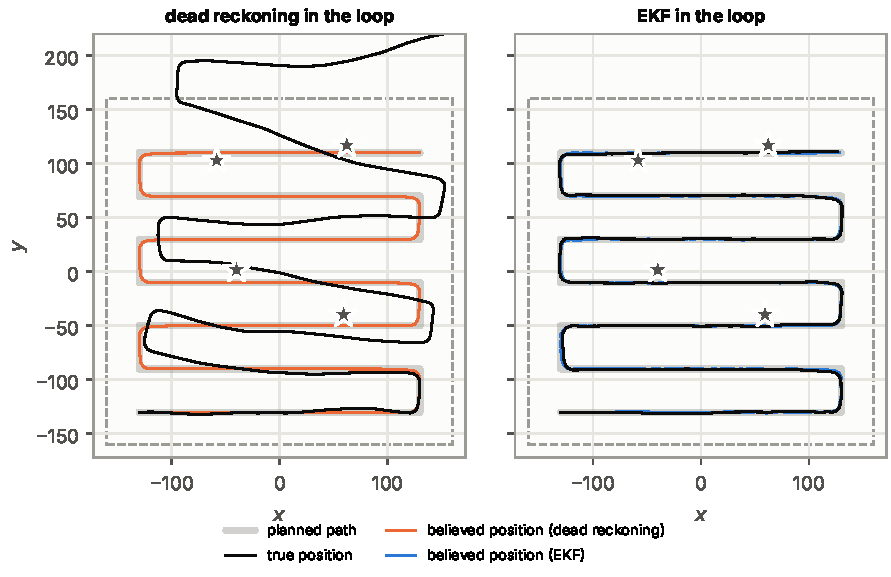
\includegraphics[width=\linewidth]{figures/ch07_closed_loop.pdf}
\caption{The filter in the loop, on a mowing pattern (seed 1). Grey: the
planned stripes. Colour: where the robot believes it is. Black: where it
really is. Left: with dead reckoning the believed path lies exactly on
the plan, while the true robot drifts and leaves the lawn. Right: with the
EKF the estimate follows the truth, so correcting the estimate corrects
the robot.}
\label{fig:closedloop}
\end{figure}

\Cref{fig:closedloop} shows the two extremes. With \emph{dead reckoning}
in the loop (the commands are integrated and no sensor is read), the
estimate is by construction where the controller wants it: the robot
believes that it follows the stripes perfectly, and nothing tells it that
it does not. With a filter in the loop, an error of the true position
shows up in the measurements, then in the estimate, and the controller
removes it. Over 10 runs:
\begin{center}
\begin{tabular}{@{}lrrr@{}}
\toprule
filter in the loop & cross-track RMS & estimation RMSE & left the lawn\\
\midrule
dead reckoning & 27.3 & 90.5 & 10/10\\
KF (compass + GPS) & 1.24 & 2.11 & 0/10\\
EKF & 0.83 & 1.18 & 0/10\\
UKF & 0.82 & 1.18 & 0/10\\
PF ($N=1000$) & 0.85 & 1.27 & 0/10\\
\bottomrule
\end{tabular}
\end{center}
Every filter keeps the robot on its stripes to within about one unit. The
estimation errors are close to those of the tracking scenario above (for
the EKF, $1.18$ against $1.16$): being in the loop does not make the filter's task
harder here. The cross-track error is smaller than the estimation error
because it counts only the part of the error that lies across the path.

Two remarks. First, in the loop the command is computed from the filter's
own estimate, hence from the measurements that the filter has received.
This is the case in which the recursion of \cref{thm:bayes} is exact,
although the controls are not fixed in advance (\cref{sec:bayesnet-mower},
complement). Second, the loop also carries the filter's failures to the
wheels: a filter that is lost, after a kidnapping or a wrong association,
steers the robot with the same confidence as before. This is the practical
reason to monitor consistency (NIS) on a real robot, and to stop when the
estimate is no longer credible.

\begin{practice}[\nb{07\_closing\_the\_loop.ipynb}, \code{control.py}]
\code{stripes\_path} builds the waypoints, \code{PathFollower} is the
controller, and \code{simulate\_closed\_loop} runs any filter of the
package in the loop and returns the run that it produced together with the
filter's estimates. \code{DeadReckoning} is the filter that never reads a
sensor. The notebook reproduces \cref{fig:closedloop} and the table, and
suggests experiments: a limited sensor range, a wrong initial pose, a
kidnapping.
\end{practice}

\section{From filtering to smoothing}
\label{sec:smoothing}

All the filters of this book estimate the \emph{current} state and then
forget the past. Yet a later measurement still carries information about
an earlier pose (\cref{sec:bayesnet-mower}, statement~(d)). Estimating the
whole trajectory from all the measurements is called \emph{smoothing}. For
the current pose of a linear-Gaussian model the two give the same answer,
so filtering loses nothing there.

As in \cref{prop:gaussnewton}, $\norm{\vect e}_A^2=\vect e\T A^{-1}\vect e$
is the squared Mahalanobis norm: the squared size of $\vect e$ counted in
standard deviations of a noise of covariance $A$.

\begin{proposition}{The Kalman filter solves a least-squares problem}{batch}
For the linear-Gaussian model of \cref{def:lgmodel}, the trajectory
$\x^\star_{0:T}$ that minimises
\[
  J(\x_{0:T})=\tfrac12\norm{\x_0-\hx_0}_{P_0}^2+\tfrac12\sum_{t=0}^{T-1}
  \norm{\x_{t+1}-F_t\x_t-B_t\uu_t}_{Q_t}^2+\tfrac12\sum_{t=1}^T
  \norm{\z_t-H_t\x_t}_{R_t}^2
\]
has $\x^\star_T=\hx_T$, the Kalman filter's estimate at time $T$.
\end{proposition}

\begin{proof}
By \cref{prop:joint}, $-\log p(\x_{0:T}\mid\z_{1:T},\uu)=J(\x_{0:T})
+\text{const}$, and $J$ is a positive definite quadratic, so the posterior
over the whole trajectory is Gaussian and its mode $\x^\star_{0:T}$ is its
mean. The mean of a marginal is the marginal of the mean, so
$\x^\star_T=\E[\x_T\mid\z_{1:T},\uu]$, which is the mean of
$\bel(\x_T)$: $\hx_T$ by \cref{thm:kf}.
\end{proof}

\begin{figure}[ht]
\centering
\begin{tikzpicture}[>=Stealth,
    var/.style={circle,draw=black!70,fill=white,minimum size=7.5mm,
      inner sep=0pt},
    fac/.style={rectangle,fill=black!75,minimum size=2.2mm,inner sep=0pt},
    meas/.style={rectangle,fill=orange!85!black,minimum size=2.2mm,
      inner sep=0pt}]
  \foreach \i/\lab in {0/0,1/1,2/2,3/3,5/T}{
    \node[var] (x\i) at (2*\i,0) {$\x_{\lab}$};}
  \node at (8,0) {$\cdots$};
  \node[fac,label={[font=\scriptsize]above:prior}] (p0) at (-1.1,0) {};
  \draw (p0) -- (x0);
  \foreach \a/\b in {0/1,1/2,2/3}{
    \node[fac] (m\a) at (2*\a+1,0) {};
    \draw (x\a) -- (m\a) -- (x\b);}
  \node[fac] (m3) at (7,0) {}; \draw (x3) -- (m3) -- (7.6,0);
  \node[fac] (m4) at (9,0) {}; \draw (8.4,0) -- (m4) -- (x5);
  \foreach \i in {1,2,3,5}{
    \node[meas] (z\i) at (2*\i,-1.1) {};
    \draw (x\i) -- (z\i);}
  \node[font=\scriptsize,right] at (10.25,-1.1) {measurement factors
    $p(\z_t\mid\x_t)$};
  \node[font=\scriptsize,above] at (5,0.45) {motion factors
    $p(\x_{t+1}\mid\x_t,\uu_t)$};
  \draw[decorate,decoration={brace,amplitude=4pt,mirror},black!60]
    (-0.4,-1.65) -- (8.4,-1.65) node[midway,below=4pt,font=\scriptsize]
    {smoothing: estimate all of them};
  \draw[decorate,decoration={brace,amplitude=4pt,mirror},black!60]
    (9.6,-1.65) -- (10.4,-1.65) node[midway,below=4pt,font=\scriptsize]
    {filtering};
\end{tikzpicture}
\caption{The factor graph of \cref{prop:joint}: one variable per pose
(circles) and one factor per term of the cost $J$ (squares): a prior,
the motion between consecutive poses, and the measurement at each pose.
A filter estimates only the newest pose and summarises the rest by its
belief; a smoother estimates the whole chain, and can still correct the
past.}
\label{fig:factorgraph}
\end{figure}

\Cref{fig:factorgraph} draws the structure of $J$. It is the Bayesian
network of \cref{fig:bayesnet} seen from the side of the cost: each
conditional distribution of the network becomes one factor, that is, one
squared term of $J$.

The cost $J$ divides by $Q_t$, which must therefore be invertible. For
the robot's motion model it is not: $Q_t=VMV\T$ has rank $2$
(\cref{prop:firstorder}). The motion term is then written with the
control noise as the unknown, $\tfrac12\norm{\bepsilon_t}_M^2$ subject to
$\x_{t+1}=f(\x_t,\uu_t+\bepsilon_t)$, which is the case announced at the
end of \cref{sec:shape}.

In the non-linear case
the equivalence between filtering and smoothing breaks. The EKF linearises
each
measurement once, at the estimate available \emph{at that time}, and
never revisits that decision, even after later measurements have shown the
estimate to be wrong. The minimiser of the same cost $J$ with $f$ and $h$
non-linear can instead be found by Gauss--Newton over the whole
trajectory, re-linearising \emph{every} past state at each iteration;
\cref{prop:gaussnewton} is the one-state, one-iteration special case. This
is \emph{smoothing}, and it is the basis of modern localisation and
mapping (SLAM): the cost is a sum of small terms, each involving a few
variables (\cref{prop:joint}), so its Hessian is sparse, and the problem
can be drawn as a \emph{factor graph} and solved efficiently even with
thousands of poses. Filtering remains the right tool when only the current
state matters and the models are nearly linear over the uncertainty, or
when the belief is multimodal and a particle filter is needed; smoothing
when the past can still be corrected and the cost of keeping it is
affordable.

The companion course \url{https://github.com/CL-BZH/vslam-course} takes
up exactly this point of view, with the same robot lawnmower as its running
example: the SLAM problem as nonlinear least squares over a factor graph,
rigid motion and Lie groups, cameras, bundle adjustment, loop closure, and
fusion with an IMU, wheel odometry and RTK-GNSS.

\begin{practice}[\nb{06\_showdown.ipynb}]
The notebook runs the four scenarios above with every filter, prints the
tables of this chapter and plots the error curves of the kidnapping and
unknown-association runs. \code{run\_filter} drives any filter of the
package over a \code{Run} and records its means, covariances and timing,
so a new filter only needs \code{predict}, \code{update}, \code{mean} and
\code{cov} to join the comparison.
\end{practice}

\begin{mower}
A practical mower uses several of these filters at once. An EKF (or UKF)
fuses wheel odometry, an IMU and RTK-GNSS for smooth, cheap tracking;
its NIS is monitored, and when it fails, or when a lift sensor reports a
kidnapping, a particle filter re-localises the mower against a map before
handing a Gaussian back to the EKF. Mapping the garden in the first
place, or localising with a camera, is a smoothing problem.
\end{mower}

\FloatBarrier
\section*{Exercises}
\addcontentsline{toc}{section}{Exercises}

\begin{enumerate}[label=\textbf{7.\arabic*},ref=7.\arabic*]
\item\label{ex:smoothvar} For the scalar random walk of
  \cref{prop:steady}, compare the variance of the filtered estimate
  $\hat x_t$ in steady state with that of the smoothed estimate of
  $x_t$ given measurements on both sides, far from the ends. Use the
  information form: what does the measurement at $t+1$ add?
\item\label{ex:addfilter} Describe the smallest change to the package
  that adds an iterated EKF (\cref{prop:gaussnewton}) to the showdown.
  Which scenario would you expect it to improve, and which not?
\item\label{ex:hybrid} Design a hybrid filter: a particle filter that
  hands over to an EKF once its cloud is unimodal, and back when the NIS
  of the EKF leaves its band. What statistic of the cloud would you use to
  decide that it is ``unimodal enough''?
\end{enumerate}

\subsection*{Solutions}

\textbf{7.1.} The filtered variance in steady state is
$P_\infty=\bar P_\infty-q$ (\cref{prop:steady}). The smoothed estimate
combines two independent sources of information about $x_t$: the past
(the filter, variance $P_\infty$, including $z_t$) and the future (a
backward filter that has not seen $z_t$; by time-reversal symmetry of the
random walk, its prediction of $x_t$ has variance $\bar P_\infty$).
Information adds (\cref{prop:information}):
$1/P^{\mathrm{s}}=1/P_\infty+1/\bar P_\infty$. With $q=0.16$ and $r=64$:
$P_\infty=3.12$, $\bar P_\infty=3.28$, and $P^{\mathrm s}=1.60$: the
smoother halves the variance, because it uses about as many measurements
from the future as the filter uses from the past.

\textbf{7.2.} Add a class \code{IEKF} that subclasses \code{EKF} and
overrides \code{update} to iterate \eqref{eq:iekf} from $\x_0=\bx$ until
the step is small, using the covariance $(I-K_iH_i)\bar P$ of the last
iterate; then add it to the list of filters in the notebook. It should
improve the uncertain start (it re-linearises at a better point, reducing
the over-confidence of \cref{fig:ekftransient}) and possibly the
identified kidnapping. It will not fix unknown data association: the
association is decided before the iterations and stays wrong, and the
belief is still a single Gaussian.

\textbf{7.3.} One possible design: compute the weighted mean and
covariance of the cloud, and the fraction of the weight within a
Mahalanobis distance $\chi^2_3(0.99)$ of the mean. If that fraction is
above, say, $0.99$ for several consecutive steps and the cloud's NEES-like
spread is stable, initialise the EKF with the cloud's mean and covariance
and stop the particle filter. When the EKF's NIS exceeds its band for
several steps (or a lift sensor fires), re-initialise the particle filter,
globally or from a wide Gaussian around the EKF's estimate. A
covariance-based test can miss two close modes; clustering the particles
(e.g.\ with a few iterations of $k$-means with $k=2$) is a more reliable,
if costlier, check.
